\section{Risultati e discussione: effetti degli elementi legnosi}
È stato osservato che il legno che non viene mobilitato dalle piene è quello posto a quote relative maggiori, ad esempio su zone di deposito o sulle isole \squarecite{Gurnell:2001-island-formation}.
\\
Ogni elemento è stato individuato tramite un pallino sulla mappa; se l'elemento è esteso su più celle delle immagini, come succede nella stragrande maggioranza dei casi per i tronchi lunghi metri e gli accumuli di legno, il medesimo elemento può essere mappato in punti diversi su immagini successive.
Questo può far sembrare che il legno si sia spostato, anche se questo deriva dalla digitalizzazione manuale (ad esempio un albero depositato su una barra può essere mappato a metà del tronco o sull'apparato radicale; se viene parzialmente sepolto da un anno all'altro la mappatura può essere diversa).
Tuttavia è possibile che un legno sia stato rimpiazzato da un altro: in questo caso considerare che l'elemento sia il medesimo non è corretto; tuttavia l'approccio consente di elaborare molti punti in poco tempo.
\\
È possibile per le digitalizzazioni degli elementi legnosi del~2010-08 e~2013-10-22 osservare se i tronchi e gli accumuli che si sono spostati sotto una certa soglia si trovano sulle quote relative più elevate.
La soglia può variare da \SIrange[range-phrase = { a }]{0.5}{2.5}{\m} ed è stata scelta valutando qualitativamente le digitalizzazione in anni successivi.
\\
I grafici in \cref{graph:legno-dem-detrended-distanza} mostrano i \emph{boxplot} dei punti che hanno il legno più vicino nella digitalizzazione successiva a distanza inferiore ad una serie di soglie; l'ultimo grafico mostra invece la quota dei punti che hanno il legno più lontano della soglia nella digitalizzazione seguente.
%
\begin{figure}
	\centering
	\tikzsetnextfilename{legno_dem_detrended_distanza}
\begin{tikzpicture}
	\begin{groupplot}[
		group style = {
			group size = 3 by 1,
			y descriptions at = edge left,
			x descriptions at = edge bottom,
			horizontal sep = 0.1cm,
		},
		width = 0.38\textwidth,
		height = 0.4\textwidth,
		xlabel = {Distanza soglia \si{[\m]}},
		%xticklabel style = {font=\tiny},
		ylabel = {Quota relativa \si{[\m]}},
		boxplot/draw direction = y,
		ymax = 0.65,
		ymin = -0.55,
		%enlarge y limits = 0.05,
		grid = major,
	]
	\nextgroupplot[
		width = 0.3\textwidth,
		title = {2010-08/2013-10-22},
		xtick = {1, 2},
		xticklabels = {$2$, $2.5$},
		] % 2010/2013
		\addplot [
		        boxplot prepared = {
		                lower whisker = -0.142529,
		                lower quartile = -0.049205,
		                median = 0.042889,
		                upper quartile = 0.189542,
		                upper whisker = 0.327826,
		                },
		        ]
		        coordinates {};
		\addplot [
		        boxplot prepared = {
		                lower whisker = -0.096515,
		                lower quartile = 0.020497,
		                median = 0.163037,
		                upper quartile = 0.245633,
		                upper whisker = 0.278409,
		                },
		        ]
		        coordinates {};
%		\node [fill = white, draw = black, anchor = north west] 
%        	at (axis description cs: 0,1) {Gurnell et al. 2018};
	\nextgroupplot[
		width = 0.55\textwidth,
		title = {2013-10-22/2014-10-31},
		xtick = {1, 2, 3, 4, 5},
		xticklabels = {$0.5$, $1$, $1.5$, $2$, $2.5$},
		] % 2013/2014
		\addplot [
		        boxplot prepared = {
		                lower whisker = 0.281042,
		                lower quartile = 0.385799,
		                median = 0.437347,
		                upper quartile = 0.528038,
		                upper whisker = 0.562563,
		                },
		        ]
		        coordinates {};
		\addplot [
		        boxplot prepared = {
		                lower whisker = -0.004163,
		                lower quartile = 0.187134,
		                median = 0.364044,
		                upper quartile = 0.468307,
		                upper whisker = 0.528088,
		                },
		        ]
		        coordinates {};
		\addplot [
		        boxplot prepared = {
		                lower whisker = -0.076253,
		                lower quartile = 0.124092,
		                median = 0.349297,
		                upper quartile = 0.458878,
		                upper whisker = 0.568133,
		                },
		        ]
		        coordinates {};
		\addplot [
		        boxplot prepared = {
		                lower whisker = -0.118472,
		                lower quartile = 0.050575,
		                median = 0.342194,
		                upper quartile = 0.451180,
		                upper whisker = 0.565715,
		                },
		        ]
		        coordinates {};
		\addplot [
		        boxplot prepared = {
		                lower whisker = -0.273404,
		                lower quartile = -0.001945,
		                median = 0.312073,
		                upper quartile = 0.446487,
		                upper whisker = 0.565771,
		                },
		        ]
		        coordinates {};
%		\node [fill = white, draw = black, anchor = north west] 
%        	at (axis description cs: 0,1) {2010};
	%------------------------------------------------------
	\nextgroupplot[
		width = 0.3\textwidth,
		title = {Legno mobilitato},
		xlabel = {Digitalizzazioni},
		xtick = {1, 2},
		xticklabels = {10/13, 13/14},
		] % punti più distanti
		\addplot [
		        boxplot prepared = {
		                lower whisker = -0.451044,
		                lower quartile = -0.118087,
		                median = 0.065396,
		                upper quartile = 0.254933,
		                upper whisker = 0.454207,
		                },
		        ]
		        coordinates {};
		\addplot [
		        boxplot prepared = {
		                lower whisker = -0.381036,
		                lower quartile = -0.136173,
		                median = 0.120033,
		                upper quartile = 0.352123,
		                upper whisker = 0.534039,
		                },
		        ]
		        coordinates {};
	\end{groupplot}
\end{tikzpicture}

	\caption[\emph{boxplot} delle quote relative dove si trova il legno mobilitato]{\emph{boxplot} delle quote relative dove si trova il legno mobilitato nelle digitalizzazioni 2010-08/2013-10-22 (per le quali non ci sono punti con distanza minore di \SI{2}{\m}) e 2013-10-22/2014-10-31; l'ultimo grafico mostra la quota relativa del legno non mobilitato, la quale è praticamente costante per ogni soglia di distanza.}
	\label{graph:legno-dem-detrended-distanza}
\end{figure}
%

All'aumentare della soglia ci sono più punti con distanza minima tra una digitalizzazione e la successiva minore della soglia stessa.
Per le digitalizzazioni 2010-08/2013-10-22 al di sotto della soglia di~\SI{2}{\m} i punti per ogni \emph{boxplot} sono molto pochi, da~3 a nessuno, e sono quindi stati scartati; il basso numero di punti può essere dovuto alle numerose ed intense piene che sono avvenute tra le due date, le quali hanno di sicuro mobilitato gran parte del legname presente.
Per le digitalizzazioni 2013-10-22/2014-10-31 ci sono~8 punti per la soglia più piccola di~\SI{0.5}{\m}, sufficienti per avere un \emph{boxplot} significativo.
\\
I legni che vengono mobilitati, cioè i punti che presentano distanza minima maggiore della soglia, mostrano tutti la stessa distribuzione per ogni soglia all'interno di ciascuna coppia di digitalizzazioni confrontate: praticamente a qualunque quota relativa un elemento legnoso può essere spostato oppure seppellito da depositi di ghiaia, così da non essere più visibile nella digitalizzazione successiva.
\\
Per il 2010-08/2013-10-22, i \emph{boxplot} dei punti con distanza superiore alla soglia si sovrappongono completamente a quelli con distanza inferiore alla soglia: non è possibile quindi avanzare altre ipotesi se non che al passaggio di un gran numero di piene e di eventi importanti il legno si sposta e che quelli che sembrano non essersi mobilitati in realtà sono stati rimpiazzati da altri elementi.
\\
Nelle mappe 2013-10-22/2014-10-31 al crescere della soglia di distanza massima i \emph{boxplot} si estendono verso quote minori, ma la mediana varia molto poco rimanendo circa costante ad una quota di~\SIrange[range-phrase = {-}, range-units = single]{3}{4}{\m}.
Inoltre c'è una discreta separazione tra i \emph{boxplot} delle distanze inferiori di~\SIrange[range-phrase = { e }]{0.5}{1}{\m} e il \emph{boxplot} del legno mobilitato.
Questi fatti fanno pensare che gli elementi legnosi individuati da quelle soglie siano i medesimi tra il~2013 e il~2014: le piccole piene avvenute ad inizio del~2014 possono aver spostato il legno a quote relative minori mentre il legno posto più in alto non è stato toccato.
Quest'ultimo ha la possibilità concreta di riprodursi vegetativamente ed essere il nucleo di formazione di nuove isole.
\\
Questi risultati riflettono le numerosi osservazioni sul campo che sono state riportate da più articoli \squarecites{Gurnell:2001-island-formation}{Gurnell:2006-omega}{Bertoldi:2009-2m}{Gurnell:2014-plants-eng}.

La crescita è un fenomeno molto più lento dell'erosione ed è controllato da più fattori, come descritto nella sezione~\ref{sec:descr-area-studio}.
\\
Si è osservato tramite il confronto tra le digitalizzazioni 2014-10-31/2015-08-13 e 2015-08-13/2017 che molti degli elementi legnosi posti a quote relative elevate nel~2013-10-22 non si sono spostati fino agli anni più recenti; si è controllato se questi hanno gettato rami e foglie e se hanno formato delle isole pioniere.
Tuttavia, sembra che non ci sia stata alcuna crescita, forse a causa di una falda troppo profonda o di un substrato troppo grossolano; qualche pianta è cresciuta, ma pare che la successione biogeomorfica sia avanzata.
Dal controllo delle mappe che rilevano l'accrescimento delle isole utilizzate nelle sezioni precedenti non è stato notata alcuna nuova isola a partire da o attorno ai punti considerati.
\\
Da una parte molte piante sono cresciute a partire da semi in zone che già nell'ortofoto del~2005-05 si stavano vegetando. Il periodo 2005/2008 è stato molto favorevole per l'espansione delle isole, come già evidenziato nella sezione precedente.
Si può ipotizzare che queste isole abbiano occupato gran parte delle zone più aggradate; così non avrebbero consentito al nuovo legno di sfruttare le aree di ghiaia nuda adatte alla crescita (\cref{fig:crescita-2005-2010-2013}).
%
\begin{figure}
	\centering
	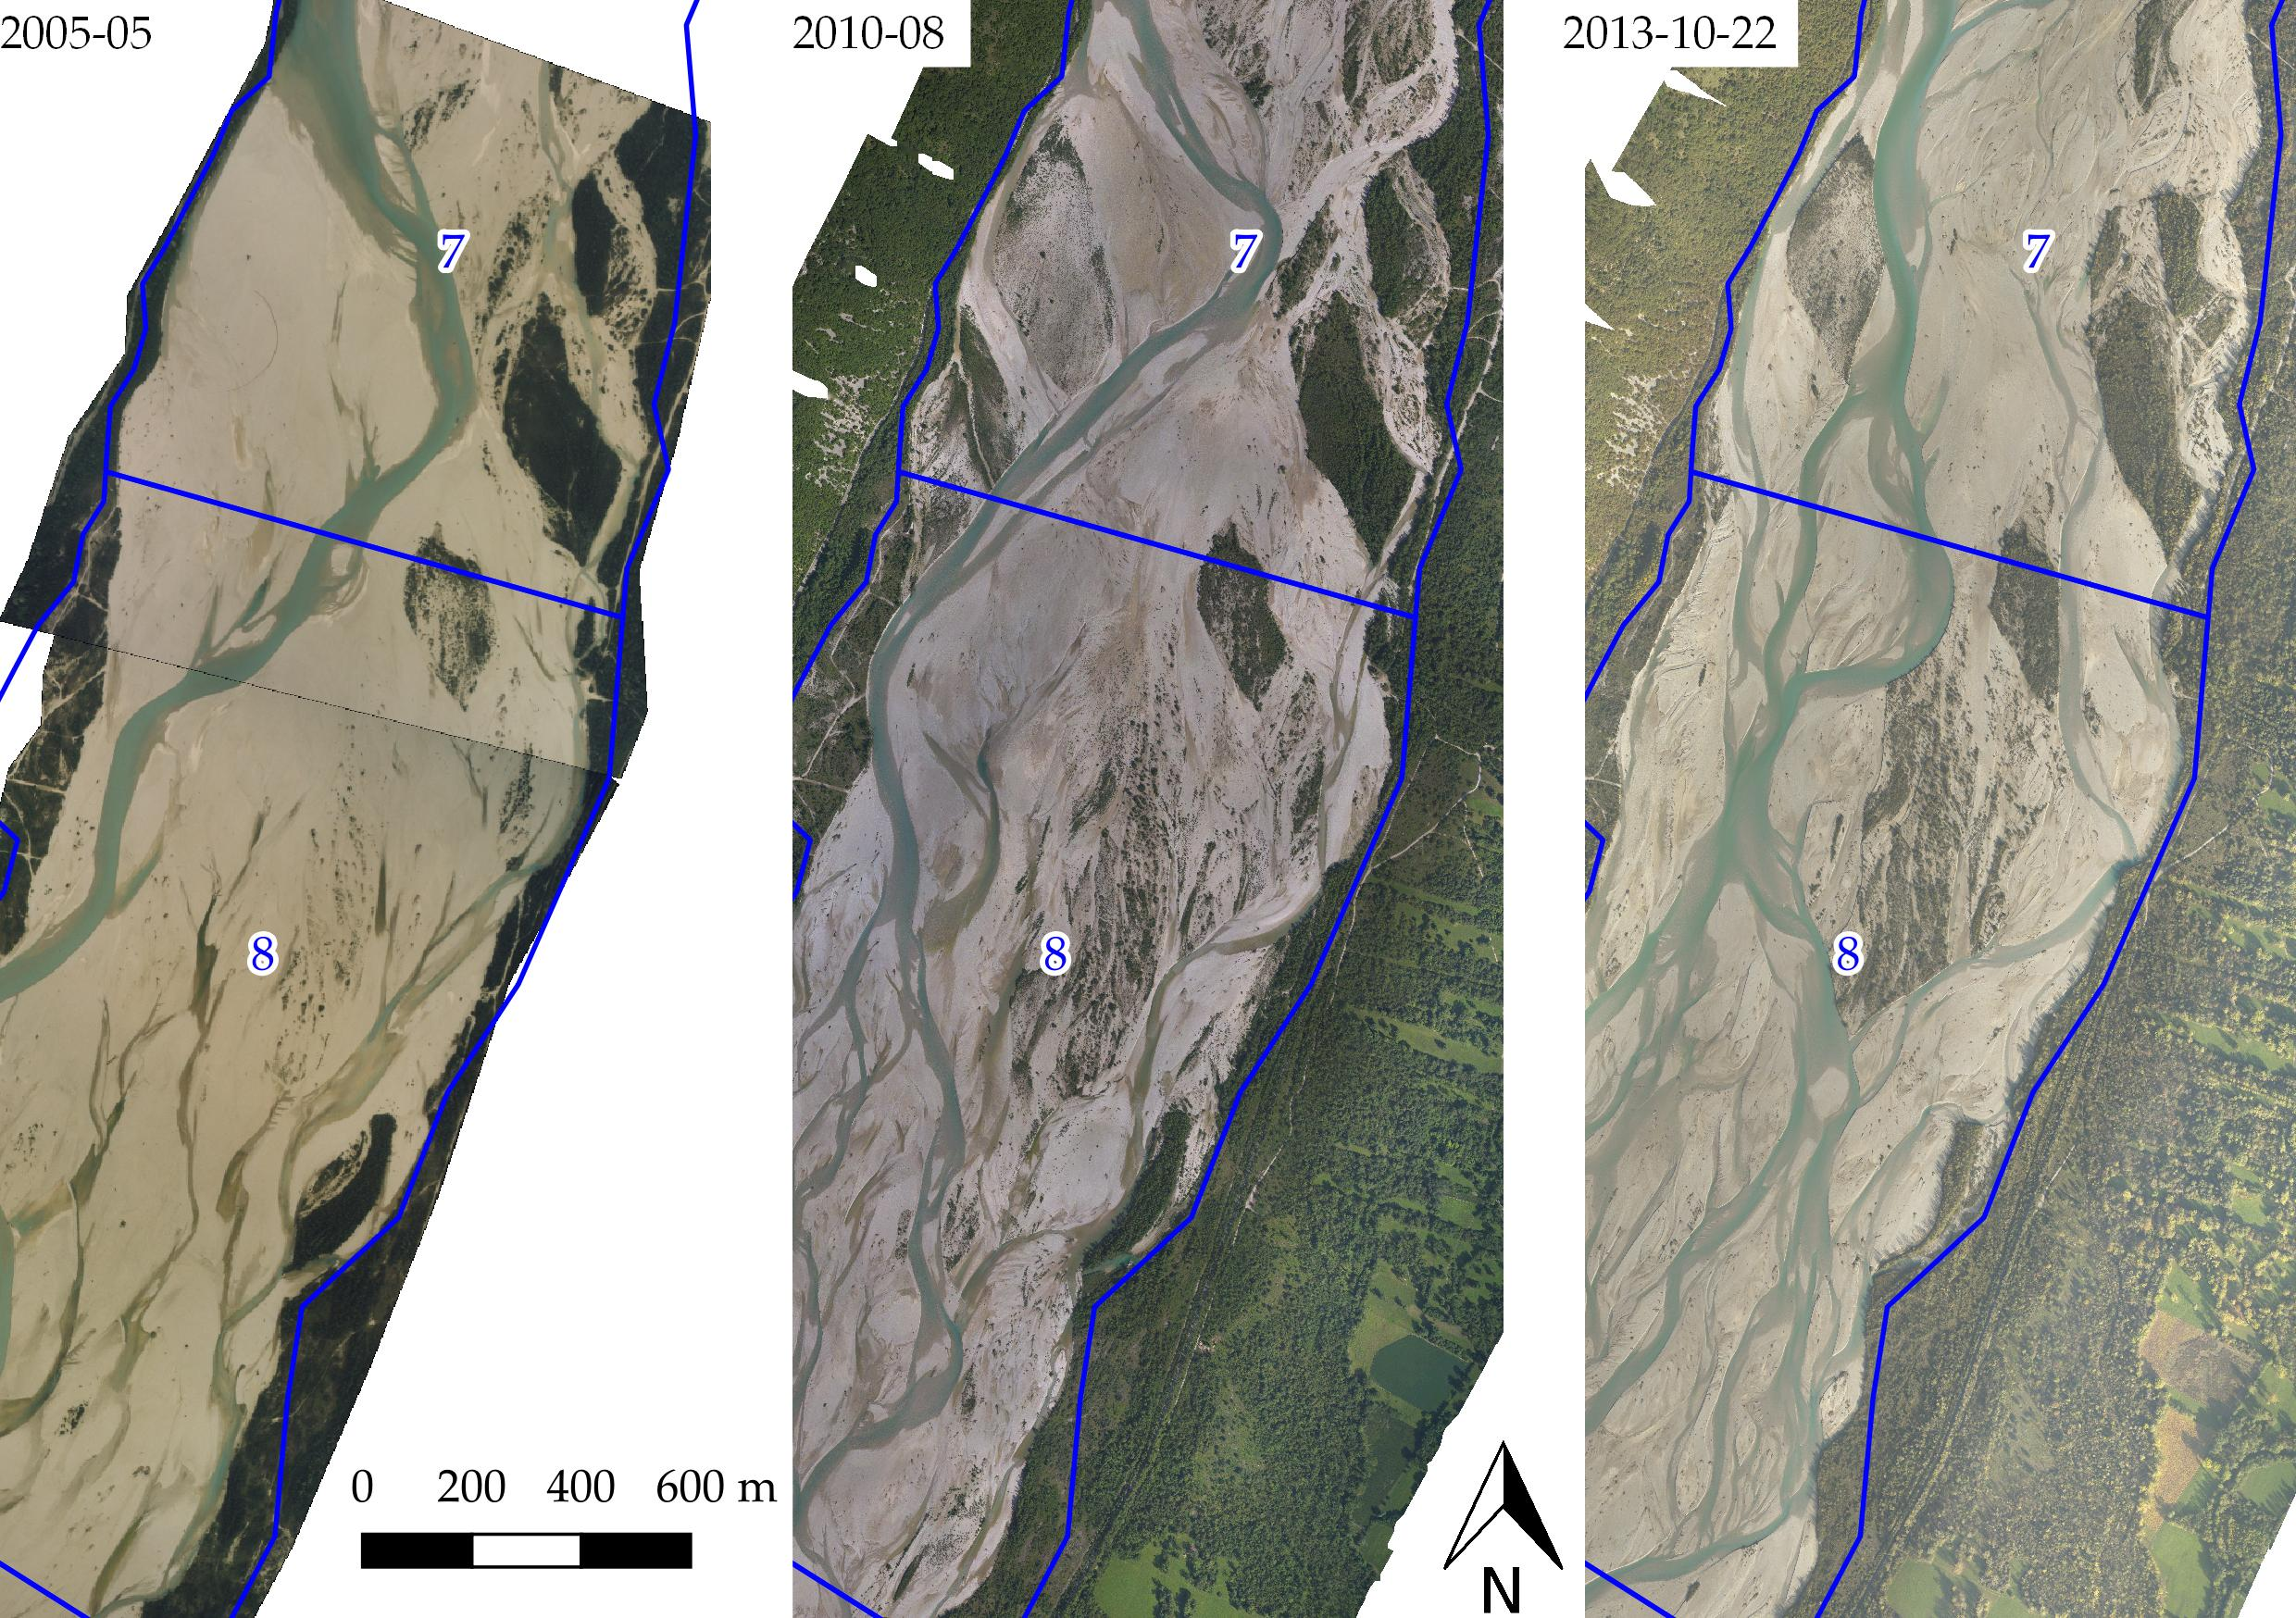
\includegraphics[width = \textwidth]{files/crescita_2005_2010_2013.jpeg}
	\caption[crescita delle isole nelle ortofoto 2005-05, 2010-08 e 2013-10-22]{crescita delle isole nelle ortofoto 2005-05, 2010-08 e 2013-10-22; si nota la forte colonizzazione di molte aree inizialmente di ghiaia nuda dal~2005-05 al~2010-08; in blu sono rappresentati i limiti della maschera computazionale divisa in tratti.}
	\label{fig:crescita-2005-2010-2013}
\end{figure}
%

I risultati mostrano che 
